\documentclass[12pt, letterpaper]{article}
\usepackage[utf8]{inputenc}
\usepackage{graphicx}
\usepackage{booktabs}

\usepackage[usenames,dvipsnames]{color}
\newcommand{\todo}[1]
  {{\scriptsize \textbf{\color{red} {#1}}}}
  
   
\title{Challenges faced in the process of knowledge transfer in an industrial environment}
\author{Mauricio Soto\\
mauriciosoto@cmu.edu
}
\date{Fall 2017}
 
\begin{document}
 
\begin{titlepage}
\maketitle


\begin{abstract}
I analyze the knowledge transfer process in several industrial contexts, corresponding to my 
previous professional experiences in industrial environments.
I contrast and compare the four different industrial experiences I had before joining the PhD program and 
how knowledge transfer played an important role in my learning process for each of these companies.
I discuss how the knowledge transfer process was handled in diverse ways in the distinct contexts I took part
of. Also how the resources and mechanisms companies have to handle knowledge transfer have an impact in the 
amount of time needed to be spent by both the newcomers and the mentors to understand the code base. 
\end{abstract}
\end{titlepage}
 
\section{Introduction}

Domain specific knowledge is one of the key assets to maintain competitiveness in 
software enterprises.
The role that this knowledge plays in the current market continues to grow, and it 
is critical for companies to be able to maintain, increase and manage their knowledge in the face 
of constant change. To sustain competitive advantages, companies must assess their knowledge resources and 
establish their knowledge strategy~\cite{civi00}. In this context, the value of knowledge transfer 
becomes a decisive factor.

Knowledge transfer is a particularly challenging problem because of the characteristics of
knowledge itself. Knowledge is distributed, ambiguous and 
disruptive~\cite{Newell06}, making its transfer a
slow and troublesome process. 
In the context of the software industry, this knowledge includes, for example: specific training in 
programming languages, tools and standard procedures used by the enterprise, as well as the
business logic required to understand the proper use and requirements of the product being built.
The social problems that occur during the knowledge transfer process are also part of the 
challenges faced, such as resistance to power/knowledge shifts or close-mindedness.

A clear example of when substantial knowledge needs to be transferred is when an existing 
enterprise opens a new branch.
Owning branches in different locations enables a pool of resources that enterprises would not be able
to obtain otherwise, such as special talents, legal benefits, or financial gain~\cite{ceruttia07}. However, 
opening a new branch is accompanied by a set of inherent challenges, such as 
difficulties in communication among team members distributed in different locations, 
cultural and language barriers, and transmitting the knowledge, culture, and mechanisms necessary for the 
coworkers in the new branch to perform their tasks adequately.

I have had the opportunity to work with diverse contexts of knowledge and culture transfer in 
an industrial environment. I will compare and contrast my experiences, with a slight emphasis on the 
latest experience I had before joining the PhD program. A large well-known enterprise was 
opening a new branch in Costa Rica and was starting to face the challenges this process encompasses.  

\section{Knowledge management and transfer}
Knowledge is one of the most important organizational resources that current enterprises possess.
The transfer of this knowledge, specially from senior to junior collaborators, 
is a key process to maintain, augment, and
make proper use of that knowledge base. 
There are continuous efforts towards creating ways to preserve knowledge in society, and software 
companies are not an exception. The concept of Knowledge Management
has gained importance in the last decades, as the process of dealing with the management 
of knowledge and its related activities. 
The main goal of these activities is to make the enterprise act as intelligently as possible to secure its viability and overall success, and
to realize the best value of its knowledge assets~\cite{wiig97}.

Organizing the process of passing down knowledge has noticeable gains, 
specially since knowledge is an increasingly important asset. Some of the benefits that come from proper management and transfer of knowledge are: Financial
Value, Operational Benefits, Business process improvement and Culture~\cite{ibrahim09}. These translate into concrete assets such as
improvements in cost, quality, cycle time, lead time, decision making and resolved complaints.

Learning is tightly connected to the knowledge transfer
process, and the learning capabilities of teams and individuals play an important role in 
this process.
There two kinds of knowledge: When you learn \textbf{about} something, referred to as \textit{explicit} 
knowledge; and when you learn \textbf{to do} something, called \textit{tacit} knowledge~\cite{cook99}. 
\textit{Cognitive learning} is when someone learns \textbf{about} a topic, as opposed to 
\textit{behavioral learning} which refers to the act of learning \textbf{to do} something.
In the case of knowledge transfer in a industrial environment, collaborators need both cognitive
behavioral learning.

When newcomers join a software project in an industrial environment, they find themselves in an
unfamiliar project
landscape, and they must become familiar with several features of this landscape.
There are three primary factors that impact newcomers'
success when facing a new project: early experimentation, internalizing structure
and culture, and progress validation~\cite{Dagenais10}. These three main factors
have a strong connection to knowledge transfer. ``Internalizing structure and culture", and 
``progress validation" are two components that require the communication and feedback 
of other team members. ``Early experimentation" is the process that requires the most 
individual work, but it is usually assisted by written knowledge transfer instances
such as code internal and external documentation.

The knowledge transfer process in an industrial context can take mainly two forms. It can be, for example,
face-to-face interactions between one or several apprentices and a mentor, or it can take the form of documentation 
(i.e. internal comments in the code, external documentation, educational videos, directives, etc). 

For the 
former, the concept of creating a safe space and providing support for selective information disclosure that
maps to the users' mental models, become a crucial part of the learning
experience. This enables collaboration between apprentice and mentor, and sharing of ideas and reflexions, 
enhancingthe overall learning process~\cite{Razavi06}. Appointing an active developer with social skills
as a mentor, enhances the learning experience. Other practices that boost the quality 
of the learning process are, for example, to appoint mentors who share recent
contextual information and who focus on related issues~\cite{Steinmacher12}. Constant interaction
and geographical proximity between mentor and apprentice also enhance communication, as well as 
practices such as openness, honesty, trust, respect and transparency~\cite{Whitworth06}. 

For the latter,
documentation is specially important when face-to-face interaction is impossible. Since face-to-face interactions
require the mentors' presence, which is usually a valuable resource, documentation usually
becomes the main source of information for the apprentice. Anecdotally, Parnas mentions that even
in software built with good design, which is already infrequent, they do not see these components being
reused if they do not have good documentation~\cite{brooks95}. Documentation is particularly important 
for the components that are intended to be reused the most~\cite{monperrus11}.

In both cases, the importance of the current collaborators in guiding the newcomers is crucial.
Face-to-face human guidance is invaluable since it is a two-way dialog, while documentation,
although extremely valuable as well, is a mechanism
where information travels in just one way and usually lacks detail~\cite{Dagenais10}.
 
\section{Work context}
Starting in 2010 and before joining the PhD program, I had formally worked for 4 different companies: Experian Credit 
Score Reporting Services (Experian), The University of Costa Rica (UCR), Rutgers University - The State University of New 
Jersey (Rutgers), and Intel Corporation (Intel). All of these companies 
have a different set of working environments and transmitted knowledge in different ways. Table~\ref{comparisonTable}
shows a summary of
these experiences. Some of the characteristics shown are: 
the time I worked for the company, the 
size of the product I was working with (measured in approximate lines of code), if the work was remote or in-office, the size of the 
team I worked with, the number of sites the team was distributed over, the main programming language I worked with,
and whether it was a part or full time position.

From this diverse group of experiences I have learned of trade offs being made in industrial environments
when it comes to knowledge transfer. I learned the impact that key attributes such as the number of members in the 
development team, the size of the project and the work location can make in the learning process of newcomers in a
software company. 

\begin{table}[] 
\centering
\caption{Comparison of 4 different experiences}
\label{comparisonTable}
\begin{tabular}{lllll}
\hline
                         & \textbf{Experian}      & \textbf{UCR}   & \textbf{Rutgers} & \textbf{Intel} \\ \hline
                         
\textbf{Worked for}      & 1 year                 & 4 years        & 9 months         & 1 year         \\ 
\textbf{Size of product} & 1M+ loc                & small products & $\sim$5k loc     & $\sim$5k loc   \\ 
\textbf{Work location}   & In-Office              & Remote         & Remote           & In-Office      \\ 
%\textbf{Team size}       & \multicolumn{1}{r}{7}& \multicolumn{1}{r}{5}& \multicolumn{1}{r}{2}& \multicolumn{1}{r}{3}\\ \hline
%\textbf{Number of sites} & \multicolumn{1}{r}{3}& \multicolumn{1}{r}{1}& \multicolumn{1}{r}{1}& \multicolumn{1}{r}{2}\\ \hline
\textbf{Team size}       & 7 developers           & 5 developers   & 2 developers     & 3 developers   \\ 
\textbf{Number of sites} & 3 sites                & 1 sites        & 1 sites          & 2 sites        \\ 
\textbf{Main language}   & Java                   & Java           & Php              & C\#            \\ 
\textbf{Part/Full Time}  & Full                   & Part           & Part             & Full           \\ \hline
\end{tabular}
\end{table}

\subsection{Experian - Credit Score Reporting Services}
In the fall of 2013, I was offered a position at Experian - Credit Score Reporting Services, as a Software Developer II in the site located in Heredia, Costa Rica.
I quickly learned that Experian was a well-known company worldwide with over 16,000
employees. Their business encompasses credit reporting, but also other products such as decision 
analytics, marketing assistance and identity theft. I also learned that we would be working mainly with two other branches: 
Costa Mesa, California, and Santiago, Chile. 

The branch in Costa Mesa was well established, with some employees having worked for over 20 years in the company. 
The Costa Rica branch (which I just joined) was the 
latest addition to this growing 
community. I was the third employee in the identity theft field (the other two employees were hired a couple of 
weeks before me). When I left the company a year later, the Identity Theft area had over 25 employees and it 
kept growing. Experian had been going through a slow process of knowledge and culture transfer and had to face
the challenges that this process comprises.

My role in the company was ``Software Developer II" which is a mid level developer. I worked with a couple
of different groups, each with a different product. In this sense, Experian was very similar to how research 
is done in academia: I worked with groups composed of collaborators with different 
backgrounds and diverse levels of expertise.

The main project I worked on was a tool for identity theft prevention, to increase the security of end users.
When end users want to check their credit score, they go to the Experian website and provide authentication
information. If the information provided is below a certain threshold of accuracy, our tool is invoked. We would collect 
information from other companies about this end user, and ask questions about personal information that only this particular
individual should know. This could include information such as: in which state does the individual have a hunting license, 
what is the color of the individual's eyes as reported in their driver's license, or what is the address of a mortgage
owned by that user.

I worked on this project for a year. Throughout that year, the process of understanding this massive million LOC 
code base was an uphill experience for me. Similar to me, new employees kept getting hired for the new Costa Rican 
branch, and they had to go through a similar learning process. My previously entailed experience falls into a large
umbrella of challenges faced by companies when dealing with knowledge transfer, including:

\begin{itemize}
  \item There is institutional knowledge that needs to be transferred to the new branch. There is not a single expert with  the 		  entirety of the necessary knowledge. Instead, knowledge is spread out among a 
  large number of different collaborators. Enough of this knowledge needs to be transmitted from the employees in the 
  older branches to the employees in the new 
  branch for them to be able to perform their work. In my experience, if I wanted to understand a particularly difficult
  section of code, I would ask a developer working on that section. This developer would tell me specifics about this 
  module in particular, but wouldn't know for example, where the module is being called or where do the parameters come
  from.
  \item The differences in pace and knowledge between the team in the well-established branch and the new branch.
  In the former, business knowledge is internalized and well understood by the employees 
  because the employees have an extensive amount of time working there. As opposed to the employees of the new
  branch who just started working for the company. 
  In the old branch, the employees usually have limited knowledge in new tools, 
  frameworks and technologies overall. We can contrast this with the team in the new branch, where the opposite is
  commonly seen: a team of young developers full of knowledge regarding the latest technologies and used to working at a 
  very high pace, but have no business knowledge for this particular company. 
  \item The team in the well established branch has a large set of BKP's (Best known practices and mechanisms), 
  which they have been using for a long time, to the point that they have forgotten the main reason
  why these are used. Trying to explain to a new set of young employees the rules that they have to follow but not
  knowing the main reason why they have to follow it, becomes really hard to understand both for the new employees
  as well for the older employees.
  \item The fact that the core business logic product, the concept of a ``credit score", is not used or known in the 
  cultural context of the new branch. In Costa Rican culture, credit scores are very rarely used. As opposed to the 
  United States where your credit score is checked if you want a cell phone plan, rent an apartment or open a bank account.
  In Costa Rica, credit scores are used mostly for long term loans such as mortgages and companies do not require your
  authorization to check it. Therefore, since most of the population does not posses a long term loan, and even if you do
  your credit score was checked without your knowledge, then credit scores are not a well-known concept in Costa Rican culture.
  \item Resistance to change by the employees in the old branch whose voice has more weight
  because of seniority. This is contrasted with the employees in the new branch, who have a vast set of new ideas 
  that can be implemented in the company, but also lack experience and knowledge regarding how the company works.
  I noticed this the most when the employees of the new branch suggested to use Jenkins to track the progress of our
  development and automate a lot of the development process. Even though we got a thumbs up to start using it and we did,
  the more senior developers would refuse to use it, because they didn't want to spend time learning to use a new tool.
  \item Difficulties introduced by location disparities such as geographical and time zone differences. These lead to 
  challenges in the development process, specially difficulties with communication and synchronization efforts.
  This was more noticeable in the mornings. We started working at 7am Costa Rican time, the team in Costa Mesa usually
  started working at 9am California time, which is 11am in Costa Rica. This usually meant that if we needed clarification
  or any kind of communication, we needed to wait about 4 hours every day to be able to interact with them.
  
\end{itemize}

\subsection{Past experiences}
It is particularly interesting to compare these different experiences because of the diversity and lessons learned
that they contribute to my understanding of knowledge transfer.

\subsubsection{University of Costa Rica}
At The University of Costa Rica, I worked as a Web Developer and then obtained a promotion to Webmaster. 
The institutional knowledge in this case was minimal.
I worked for a research center, with a small team of developers. We constantly got requirements to build small products 
or implement changes to existing products. These tasks usually took between a month to six months to get built.

The previous Webmaster was a single person who knew the high level details for most the products built. He possessed, 
to a large extent, the knowledge necessary to perform properly as a Webmaster in this context.
In this case, the knowledge transfer experience I had was about three hours with this previous Webmaster. He very kindly
indicated to me the knowledge he though was necessary for me to perform well, while I asked him the questions I could 
think of. The biggest limitation in this experience was the time constraint. I had only one meeting with 
this person. Further on, if some other question came to mind, or if I stumbled upon another problem, the knowledge
transfer process would be over by then.

Ultimately three hours of training was not quite enough for a position that I held for four
years. It quickly became a very challenging experience for me, mostly because the majority of the learning had to be done 
by myself. This presented the steepest learning curve of all my experiences. The 
majority of knowledge I obtained was not provided by anyone within the company, but rather via by third party
sources or by my own experimentation. For example, we used several different frameworks and plug-ins. 
I had to look for and read the documentation of 
these frameworks and plug-ins to understand how they worked. When I couldn't find documentation to read, I relied
on other learning mechanisms such as modifying the source code and re-running it to compare its behavior
before and after the changes where performed. 

Unlike my other experiences, in this one the company had a very weak knowledge transfer mechanism.
This resulted in a lot of time spent by the newcomers looking for knowledge themselves that was not passed down to them. 
The newcomers took much longer to be able to obtain knowledge that was already present in previous developers,
and could have been learned in a more straightforward way if the knowledge was properly handed down to them 
in the form of documentation or face-to-face.

\subsubsection{Rutgers University}
The second experience I will talk about was when I worked for 9 months as a Web Developer in Rutgers University, The
State University of New Jersey. This is a interesting experience to contrast with the others because the knowledge 
transfer experience was written, not verbal. The code was really well documented, but the person who had 
written the comments had already left the position. Having written documentation was advantageous because 
I could access it where/whenever it was most convenient for me. But it does not have the dialog that face-to-face
mechanisms provide, which is particularly helpful when I had doubts not covered by the documentation. 

When I applied for this position, I was first interviewed by the director of a recreational facility, 
a non-technical person. He broadly explained to me that I was going to 
perform several changes to a program used by the recreational facility for record keeping,
test taking, etc. Once I started the job, the director gave me the password to the server and told me to 
get myself familiarized with the program (a 5,000 line PHP program). At this point I had to go through
the program understanding what it was supposed to do, reading the comments, running it in different ways, making small 
changes to the 
functionality and re-running it to confirm that I was properly understanding the functionality, and after a couple of 
weeks of doing this I was able to understand generally how the program worked and how to perform the changes I was asked
to implement.

\subsubsection{Intel}
Finally, I worked at Intel Corporation, where I was hired
as a Software Developer in February of 2012. In this opportunity, I joined a group of 3 people (myself included):
two developers (located in Costa Rica) and one project manager (located in Arizona). Both branches, 
had existed for over 20 years. The working culture had been well assimilated and internalized. 
This helped softened my immersion into the work environment since I had to only adapt to the already
existing working culture(as opposed to Experian where we were creating a culture from scratch).

One important factor that made my transition more pleasant regarding knowledge transfer was that 
the other developer I was working with was knowledgeable. He knew the technologies and processes
being used in this team very well, and was able to explain to me with as much detail as 
needed how to perform a task I was not familiar with. 

Second, he was available. We worked in the same cubicle and when I needed further explanation of any given 
task we would have the location proximity and he would always take a couple of minutes of his time
to further explain unfamiliar concepts to me. Also, since we were regular co-workers, knowledge transfer did not have a
time limitation (as opposed to my experience in the University of Costa Rica), so knowledge could flow in my
direction very naturally. When I was starting, I needed a lot more help and feedback about my work. 
Later, needed less and less, 
until most of the knowledge I needed was assimilated, with the exception of very sporadic questions. 

In my opinion, this was the best knowledge transfer experience I had of the four. This is based on
several factors:
\begin{itemize}
  \item The presence of a well-balanced set of documentation and an expert
  \item The fact that the expert was both knowledgeable and available
  \item The team I was joining was well-established, and had been working together for several years
  \item Newcomers had to only adapt to the already existing working culture, not create one from scratch
\end{itemize}

\section{Reflection}

In my experience, a hybrid approach between two- and one-way knowledge transfer is best.
This is the best and fastest way to get the newcomers to adapt and understand
a new landscape. Not all forms of documentation and face-to-face time
are equally important in an industrial environment. For example, in the experiences where I had a good balance between documentation and face-to-face time
(such as at Intel), I was able to learn much faster and assimilate the code than I could when
I had only documentation (Rutgers) or very limited face-to-face interactions with the mentors (Experian and 
UCR). 

Previous studies have focused on the difference between explicit knowledge and tacit knowledge(learn about 
something or learn to do something)~\cite{cook99,civi00}. Both of these types of knowledge are important from a software
engineering perspective. I have focused on the differences between knowledge that is 
acquired through one-way communication or two-way communication. The importance of this difference comes
mainly because
documentation(one-way communication) is a common practice in software engineering, 
and mentors(two-way communication) are usually senior developers 
whose time is highly valuable. 

I have also validated with my personal experience key insights from previous literature. 
For example, I have observed that early experimentation (UCR and Rutgers) and progress validation (Intel) are key features
in the learning process of software projects~\cite{Dagenais10}. I have also witnessed the advantages of 
learning from an active developer with social skills~\cite{Steinmacher12}
and geographical proximity~\cite{Whitworth06} (Intel and Experian). 

\subsection{One-way communication}
I have observed that proper internal documentation is the most 
important of all the forms of documentation for new developers to understand the purpose of the code they will
be working with. This includes meaningful names for classes, 
methods and variables, clean code, and developer written
comments.

The importance of this particular kind of documentation comes from the fact that it is immediate.
The newcomer will go through the code to try to understand it. When the newcomer does not understand 
a particular section of code, the first thing the newcomer will look for is code comments. 
If such comments address the doubts, the knowledge transfer will be immediate and effective.

Unfortunately, in my experience, developer written comments are extremely rarely updated, which results in 
comments that do not match what the code is currently doing. Throughout all my experiences 
I could see outdated comments on a daily basis. It was less likely when using software that is 
meant to be reproduced and understood by other developers(e.g., in frameworks). In all other cases,
where understandability was not a priority, outdated comments were a common problem.

This leads to newcomers not 
trusting the comments to understand what the code is doing because there is a discrepancy and a lack of 
constance between what the developer written comments say the code does and what the code actually does. 
Outdated documentation is in general a well known problem in software maintenance and this is a scenario
where we can see in a very clear way the impact of this problem, since it interferes and hinders vastly the 
knowledge transfer process and the learning experience of the newcomers.


\subsection{Two-way communication}
Regarding two-way communication between newcomers and mentors, in my experience, this is usually much less frequent and
represents a much smaller section of the knowledge transfer process. One of the main reasons behind this is that
senior developer's time is a highly valued asset which must be used in high priority tasks, and usually
the knowledge transfer process does not qualify as a high priority tasks in industrial environments. 

In my experience, this kind of knowledge transfer is less necessary when the documentation in the project is of high
quality and the newcomer can rely on this to obtain knowledge about the project (meaningful variable, class, and 
method names, updated internal documentation, etc). As documentation quality decreases, the need for a mentor increases.
This can be described
as an inversely proportional relationship between the quality of the documentation in the project and the 
time needed to be spent by both the mentor and the newcomer in face-to-face communication.

In my experience at Rutgers, for example, the internal documentation of the project was of high quality. Therefore
I was able to understand all the necessary code to perform my tasks properly without ever needing two-way 
communication. As opposed to my experience at Experian, where the documentation was of low quality, therefore
I needed much more mentorship.

Figure~\ref{graph1} represents this relationship between documentation quality and portion learned by
one/two-way communication. Projects in an industrial environment fall somewhere in between this spectrum 
depicted by Figure~\ref{graph1}. In the far left we have projects with high quality documentation where the vast
majority (or even all) the knowledge required by the newcomers to perform their tasks will come from the 
documentation itself. On the far left, we have the opposite: projects with low quality documentation, where most 
of the knowledge required by the newcomer will have to come from conversations with other developers since
the knowledge that the newcomers can obtain from the documentation is minimum.


\begin{figure}[h]
    \centering
    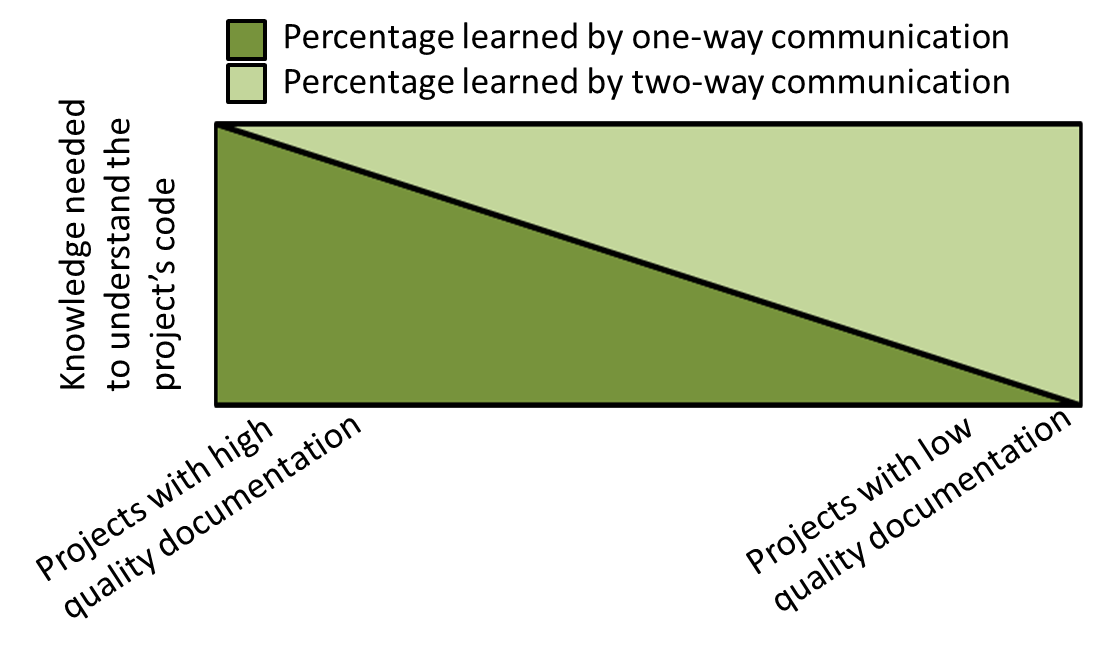
\includegraphics[width=0.85\textwidth]{Graph1}
    \caption{Percentage of one-way and two-way communication required for different types of projects with high and low quality documentation}
    \label{graph1}
\end{figure}






\section{Conclusion}

In my experience working with several different contexts of knowledge transfer in an industrial environment
I can conclude that there are two major ways of transferring knowledge from mentors to newcomers: One-way
and two-way communication. One-way communication is usually perceived in the form of documentation and it 
is characterized by the fact that information flows in only one direction. From my experience, the most 
important of the several different kinds of documentation, is the internal documentation which encompasses
names of classes, variables, methods, and developer written comments. The importance of this comes from
the immediateness of this kind of documentation to satisfy doubts the newcomers may have, and also because
it is the most commonly used source of information by newcomers. Two-way communication is needed in a inversely 
proportional manner to the quality of said documentation.

Some high level factors that can highly improve the learning experience of newcomers when joining a new software 
project are:
\begin{itemize}
  \item The presence of both documentation and an expert, with emphasis in the former
  \item Knowledgeable and available mentor(s)
  \item As long as possible, include newcomers into already existing teams with an already defined work culture 
\end{itemize}

I can derive from this information that applying best practices from code maintenance literature such as 
using meaningful names for classes, variables, and methods in the software being built, and constantly updating
the developer written comments is optimal for the knowledge transfer process in newcomers. Therefore making
the need for two-way communication between newcomers and mentors minimal. This is also advantageous for the
company since mentors tend to be more senior developers and the time that mentors spend mentoring newcomers
is time they are not creating new products or fixing important errors, tasks that usually have a higher priority
in industrial environments.

\bibliographystyle{abbrv}
\bibliography{sigproc}  % sigproc.bib is the name of the Bibliography in this case
% You must have a proper ".bib" file
%  and remember to run:
% latex bibtex latex latex
% to resolve all references

 
\end{document}